\hypertarget{architecture}{%
\section{Architecture}\label{architecture}}

Most of the architectures today are based on the \textbf{John von
Neumann-Architecture}. \emph{The programming language C is an
architecture as well.} Most of the processors are based on registers,
like the RISC-V or the Intel x64.

\hypertarget{history}{%
\subsection{History}\label{history}}

\textbf{1930 $\lambda$-Calculus (Former Programming Language}

Very minimalistic and fundamental of $\lambda$ Functions today. These are
anonymous functions.

\textbf{1937 Alan Turing with the Turing Machine (First model of
computer)}

Actually just a state machine on tapes with some I/O

\textbf{1940 - John von Neumann with his architecture}

\hypertarget{equivalent}{%
\subsection{Equivalent}\label{equivalent}}

One Architecture emulates the other Architectures

Given architectures A and B A(B):\\
Architecture A emulates architecture B. \textbf{Equivalent means: A(B)
and B(A) $\Rightarrow$ Both can emulate the other.}

\begin{tcolorbox}[colback=red!5!white,colframe=red!75!black]
e.g. Windows(Linux) and Linux(Windows) Both systems emulates the other. They are equivalent. 
\end{tcolorbox}

\hypertarget{the-church-turing-thesis}{%
\subsection{The Church-Turing Thesis}\label{the-church-turing-thesis}}

This thesis states, that every machine (architecture) is a computer. And
it is not possible to build another machine, which is more intelligent
than a computer.

\clearpage
\hypertarget{john-von-neumann-architecture}{%
\subsection{John von Neumann
Architecture}\label{john-von-neumann-architecture}}

There is generally the memory, which is the passiv component and the
CPU, which is the active component.

\begin{figure}[H]
\centering
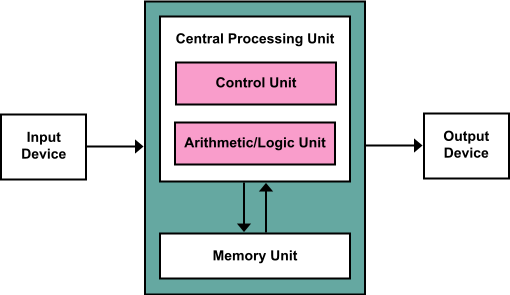
\includegraphics[width=0.6\textwidth]{figures/vonNeumann.png}
\caption{von Neumann Architecture}
\end{figure}

\hypertarget{memory}{%
\subsubsection{Memory}\label{memory}}

The memory holds the data of the machine. It can be referred and
accessed by addresses.

\hypertarget{cpu}{%
\subsubsection{CPU}\label{cpu}}

The CPU modifies the data in the memory with read and write operations.
The data read out of the memory can also be instructions.

\hypertarget{bottleneck}{%
\subsubsection{Bottleneck}\label{bottleneck}}

The architecture's advantage is that it is very easy. But the bottleneck
is the cpu. Every memory-change has to go through the CPU because the
CPU is the only active part in this architecture.

\hypertarget{main-concern}{%
\subsection{Main concern}\label{main-concern}}

\textbf{Keep} the simple but inherently slow \textbf{John von Neumann}
architecture, but \textbf{make it fast as possible} and \textbf{cheap as
possible}.

\clearpage
\hypertarget{particular-architectures}{%
\subsection{Particular Architectures}\label{particular-architectures}}

\hypertarget{the-language-c}{%
\subsubsection{The language C}\label{the-language-c}}

\begin{itemize}
\tightlist
\item
  Based on John von Neumann architecture
\item
  emulated by i386 and RISC architectures
\end{itemize}

\hypertarget{risc-v}{%
\subsubsection{RISC-V}\label{risc-v}}

\begin{itemize}
\tightlist
\item
  Based on John von Neumann architecture
\item
  Implementation of RISC
\end{itemize}

\hypertarget{intel-64}{%
\subsubsection{Intel 64}\label{intel-64}}

\begin{itemize}
\tightlist
\item
  Based on John von Neumann architecture
\item
  Implementation of CISC
\end{itemize}

\clearpage